\section{Infrastructure as a Service -- OpenStack}
\begin{itemize}
	\item main services:
	\begin{itemize}
		\item Compute: Nova, central computation
		\item Identity: Keystone, \textbf{authentication}, generate \textbf{token} for subsequent calls
		\item Image: Glance, base image selection for VM (\textbf{template for VM})
		\item Networking: Neutron, determine networking \textbf{rules}, allocate \textbf{network resources}
		\item Dashboard: Horizon
		\item Block storage: Cinder, allocate \textbf{volume}
	\end{itemize}
	\item Design concepts:
	\begin{itemize}
		\item Goal: scalability (horizontal), elasticity
		\item \textbf{asynchronous} communication: message \textbf{queues}
		\item \textbf{decentralized} data management: each microservice has its \textbf{own database}, accepts \textbf{eventual consistency}
		\item \textbf{distribute} everything: distributed into microservices, communication through APIs
	\end{itemize}
	\item Architecture:
	\begin{figure}[H]
		\centering
		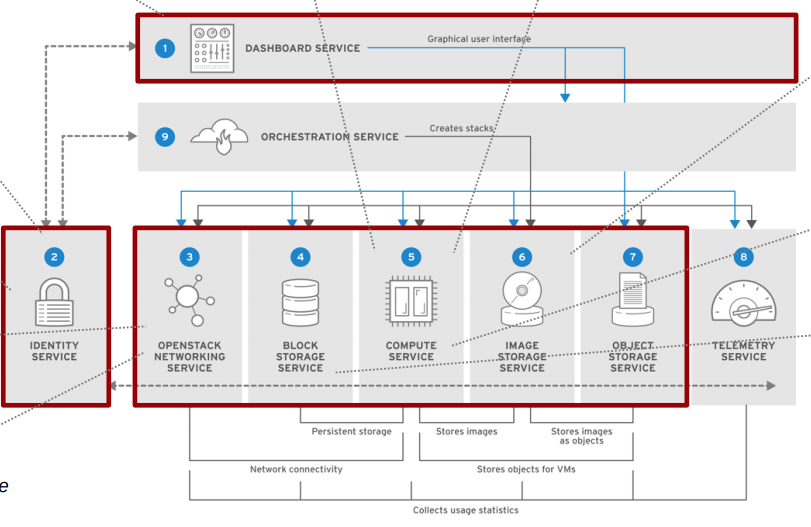
\includegraphics[width=\textwidth]{openstack.png}
	\end{figure}
\end{itemize}

\subsection{Identity Management}
\begin{itemize}
	\item provides authentication credential validation and data
	\item generates \textbf{authentication tokens} that enable clients to access OpenStack services REST APIs.
	\item clients obtain this \textbf{token} and \textbf{URL endpoints} for other service APIs.
\end{itemize}

\subsection{Compute Service}
\begin{itemize}
	\item manage and provision \textbf{virtualized server resources}: CPU/memory/disk/network
	\item VM management: start/stop/reboot/terminate
	\item communication with other services: image, identity, network, storage services
	
\end{itemize}

\paragraph{components:}
\begin{itemize}
	\item Nova API: interface to create instances
	\item RabbitMQ and compute database : provides communications hub and manage data persistence
	\begin{itemize}
		\item Message \textbf{Queue}(MQ): pass messages between services \textbf{asynchronously}
		\item compute database: \textbf{store} build-time and run-time \textbf{states}, available instance types/in use, available networks etc.
	\end{itemize}
	\item Scheduler: determines \textbf{allocation of physical hardware} to virtual resource using \textbf{series of filters}
	\item \textbf{compute node}: \textbf{management of all interactions} with individual endpoints providing computing resource
\end{itemize}

\subsection{Network, Block Storage and Image Storage}
\begin{itemize}
	\item network: manage \textbf{networks, ports, attachments on infrastructure} for virtual resources
	\item block storage: 
	\begin{itemize}
		\item create and manage \textbf{lifecycle of volumes}
		\item respond to \textbf{read and write requests} sent to block storage to maintain states
		\item \textbf{backup} volumes
	\end{itemize}
	\item image storage:
	\begin{itemize}
		\item storage in \textbf{independent} image \textbf{database}	
		\item accept API calls for \textbf{image discovery, retrieval and storage}
	\end{itemize}
	
\end{itemize}


\subsection{Server Creation Workflow}
\begin{itemize}
	\item Nova Client gets \textbf{token} from Identity Management service.
	\item After \textbf{authentication}, Nova API \textbf{sends request} of launching instance \textbf{into Message Queue}
	\item Nova scheduler \textbf{subscribes request} and \textbf{allocate resources using filtering}
	\item Nova compute communicates with Image service, Network service, block storage service to \textbf{get image, allocate network and storage}.
	\item Nova compute starts instance.
\end{itemize}


\section{Infrastructure as a Service -- Microsoft Azure}
\begin{itemize}
	\item \textbf{company-oriented} service
	\item services:
	\begin{itemize}
		\item Azure Virtual Machines
		\item Azure Virtual Network: connects \textbf{VMs and services}, connect \textbf{cloud resources with on-premise resources} through \textbf{Internet} via VPN.
		\item Azure ExpressRoute: connects \textbf{cloud resources and on-premise resources} via \textbf{dedicated lines}.
	\end{itemize}
	\item \textbf{Traffic Manager}: distribute resources to either Azure or on-premise data centers -- different service endpoints.
	\item \textbf{Resource Manager}: management as a \textbf{group}. Resource allocation defined in \textbf{template} with version control. 
\end{itemize}